\documentclass[11pt]{article}
\usepackage[margin=1in]{geometry}
\usepackage{booktabs}
\usepackage{graphicx}
\usepackage{hyperref}
\usepackage{amsmath,amssymb}
\usepackage{amsthm}
\usepackage{xcolor}
\usepackage{pgfplots}
\graphicspath{{figs_dynamics/}}
\pgfplotsset{compat=1.18}
\newtheorem{finding}{Finding}

\title{Memory Dynamics in Production Multi-Agent Systems:\\
A 30-Day Longitudinal Study of Shared Agent Memory}

\author{Anonymous}

\begin{document}
\maketitle

\begin{abstract}
Multi-agent AI systems increasingly share persistent memory, but no published study has characterized how shared agent memory evolves in production. We present a 30-day longitudinal study of a production multi-agent memory system serving 15 AI clients through a shared SQLite database (3,000 logged operations, 1,957 active memories, 7,375 entities). We report five findings: (1)~memory type predicts correction rate: procedural memories are corrected at a 91.5\% rate, over 11$\times$ higher than decisions (8.2\%); (2)~81.7\% of cross-agent fact pairs exhibit polarity clashes, yet only 0.044\% of cross-source entity pairs survive entity-level filtering as genuine temporal contradictions---a 1{,}857$\times$ reduction from the raw fact-pair clash rate to the entity-pair contradiction rate that quantifies the entity-resolution challenge; (3)~memory corrections cluster: a single system-mediated consolidation event accounts for 262 of 349 corrections (75.1\%); (4)~the injection coverage ratio is 0.48\%: the system stores 209$\times$ more content than can be presented to the LLM per turn; (5)~the 14.9\% of corrections that are cross-agent cause disproportionate downstream harm (86\% answer divergence) compared to self-corrections (0.7\% divergence). These findings suggest that memory system design should prioritize type-aware retention policies, entity-resolution quality, and cross-agent conflict interception.
\end{abstract}

\section{Introduction}
\label{sec:intro}

Multi-agent AI systems accumulate persistent memory across sessions and clients. As these systems move from research prototypes to production deployments, the dynamics of shared memory---how memories are created, corrected, and retired over time---become a critical operational concern. However, no published work has measured these dynamics in a real production environment.

Existing agent memory papers evaluate on static benchmarks (LongMemEval~\cite{wu2024longmemeval}, LoCoMo~\cite{locomo2024}) that test retrieval accuracy at a single point in time. They do not capture the temporal dynamics: how quickly do memories become stale? What fraction of stored content can actually be retrieved per turn? Do different types of memories age at different rates?

We present a 30-day longitudinal study of a production multi-agent memory system (MemTether~\cite{memtether}), which serves 15 AI clients through a single shared SQLite database with file-level pointer sharing. During the study period, the system recorded 3,000 operations (2,273 writes, 87 organic corrections (the remaining 262 were system-mediated consolidation), 200 retirements), managed 1,957 active memories across 7,375 entities, and processed 349 supersession events.

Our contributions:
\begin{enumerate}
\item The first longitudinal measurement of shared agent memory dynamics in production (30 days, 15 clients, 3K operations).
\item Discovery that memory type predicts correction rate: procedural memories have a 91.5\% correction rate, over 11$\times$ higher than decisions (8.2\%), suggesting type-aware retention policies.
\item Quantification of the entity-resolution challenge: 81.7\% of cross-agent fact pairs exhibit raw polarity clashes, but only 0.044\% are genuine temporal contradictions after filtering---a 1,857$\times$ false-positive rate.
\item Measurement of the injection coverage ratio (0.48\%): memory systems store two orders of magnitude more content than can be retrieved per turn, making retrieval quality the binding constraint.
\item Demonstration of a power-law harm distribution: the 14.9\% of corrections that are cross-agent cause 86\% downstream answer divergence, while the 81.4\% that are self-corrections cause only 0.7\% divergence.
\end{enumerate}

\section{Background}
\label{sec:background}

MemTether is a local-first agent memory system that enables multiple AI clients on the same machine to share a single SQLite database via NTFS junctions (Windows) or symbolic links (macOS/Linux). Each memory is stored as a typed row with bi-temporal timestamps (\texttt{valid\_from}/\texttt{valid\_to} for real-world validity, \texttt{recorded\_at}/\texttt{invalidated\_at} for system awareness), source attribution, and a Q-value for reinforcement learning from use.

Memories are classified into five types: \texttt{fact} (factual assertions), \texttt{decision} (choices made), \texttt{experience} (observations from interactions), \texttt{procedure} (how-to knowledge), and \texttt{incident} (error reports and anomalies). At write time, a predicate extractor parses each memory into (entity, attribute, polarity) triples and stores them in a \texttt{fact\_entities} index table.

When an agent corrects a previously stored fact, the \texttt{correct()} operation creates a supersession edge in a directed acyclic graph, marking the old fact as \texttt{superseded} with explicit validity boundaries. Every operation is logged to an append-only \texttt{audit\_log} with hash-chained anchors for tamper evidence.

\section{Methodology}
\label{sec:methodology}

\subsection{Production Environment}

Table~\ref{tab:deployment} summarizes the production environment.

Our study covers a single-machine production deployment from 2026-09-13 to 2026-10-14 (32 days, truncated to 30 for analysis). The system serves 15 distinct AI client sources through a shared \texttt{memory.db} file. Each client connects via MCP (Model Context Protocol) and writes memories with source attribution. The deployment runs on a single Windows machine (Intel CPU, 32\,GB RAM) with SQLite in WAL mode for concurrent read-write access.

\begin{table}[h]
\centering
\caption{Production deployment summary.}
\label{tab:deployment}
\begin{tabular}{lr}
\toprule
Metric & Value \\
\midrule
Study duration & 30 days \\
Distinct client sources & 15 \\
Total logged operations\footnote{Includes audit\_log entries (writes) and read tracking events; does not include raw \texttt{use\_count} increments which are tracked per-row. The unified system paper reports 31K+ total operations including 28,807 read operations (sum of use\_count) over the 30-day window.} & 3,000 \\
Active memories & 1,957 \\
Superseded memories\footnote{386 rows have status=superseded; 349 supersession edges connect them. The difference arises from multi-step chains where one edge supersedes a fact that was itself already superseded.} & 386 \\
Retired memories & 200 \\
Distinct entities & 7,375 \\
Multi-source entities & 1,580 (21.4\%) \\
Supersession events & 349 \\
\bottomrule
\end{tabular}
\end{table}

\subsection{Measurement Method}

We extract three data sources from the production database:

\begin{itemize}
\item \textbf{Audit log}: Every operation (remember, correct, retire, search) is recorded with timestamp, agent identity, and operation type. We use this for operation-level statistics and temporal analysis.
\item \textbf{Supersessions table}: Each correction creates an edge (old\_uid, new\_uid, reason, ts). We use this for memory lifetime analysis and correction pattern classification.
\item \textbf{Fact-entities index}: Each memory is linked to zero or more named entities with polarity. We use this for cross-agent overlap analysis and contradiction detection.
\end{itemize}

All measurements are computed directly from the SQLite database using SQL queries and Python analysis scripts. The database is read-only during analysis to avoid perturbing production.

\section{Findings}
\label{sec:findings}

\subsection{Finding 1: Memory Type Predicts Correction Rate}
\label{sec:type-rate}

\begin{table}[h]
\centering
\caption{Correction rate by memory type. Procedural memories are corrected at 11$\times$ the rate of decisions.}
\label{tab:type-correction}
\begin{tabular}{lrrr}
\toprule
Memory type & Total & Corrected & Correction rate \\
\midrule
Procedure & 129 & 118 & 91.5\% \\
Incident & 289 & 49 & 17.0\% \\
Experience & 426 & 46 & 10.8\% \\
Fact & 1,333 & 139 & 10.4\% \\
Decision & 413 & 34 & 8.2\% \\
\bottomrule
\end{tabular}
\end{table}

\begin{figure}[h]
\centering
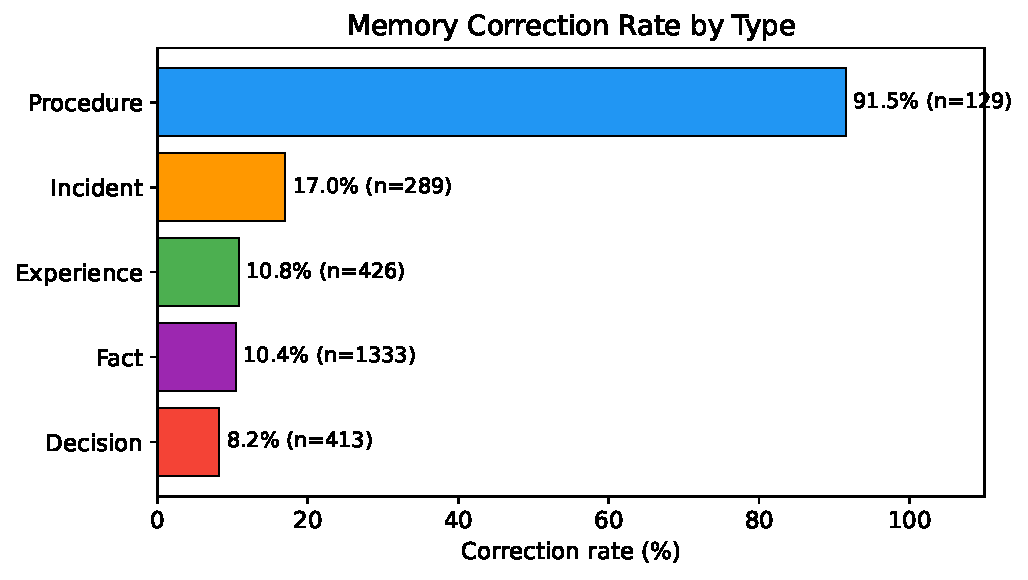
\includegraphics[width=0.8\textwidth]{fig1_type_correction.pdf}
\caption{Memory correction rate by type. Procedural memories (91.5\%) are corrected at over 11$\times$ the rate of decisions (8.2\%).}
\label{fig:type-correction}
\end{figure}

Figure~\ref{fig:type-correction} and Table~\ref{tab:type-correction} show the 11$\times$ difference between procedural and decision correction rates; this has a clear explanation: procedures describe \emph{how to do things} (tool configurations, deployment steps, API usage patterns), and these change as software is updated. Decisions describe \emph{why choices were made}, and the rationale for a decision does not change even when the implementation changes. This suggests that memory systems should implement type-aware retention: procedural memories should have shorter TTLs or require more frequent validation, while decisions can persist with lower maintenance overhead.


\subsection{Survival Analysis}
\label{sec:survival}

We apply Kaplan--Meier survival analysis to quantify memory lifetime, treating correction (supersession) as the event of interest and treating still-active memories as right-censored observations ($n{=}2{,}309$ total: 349 events, 1{,}960 censored).

\begin{figure}[h]
\centering
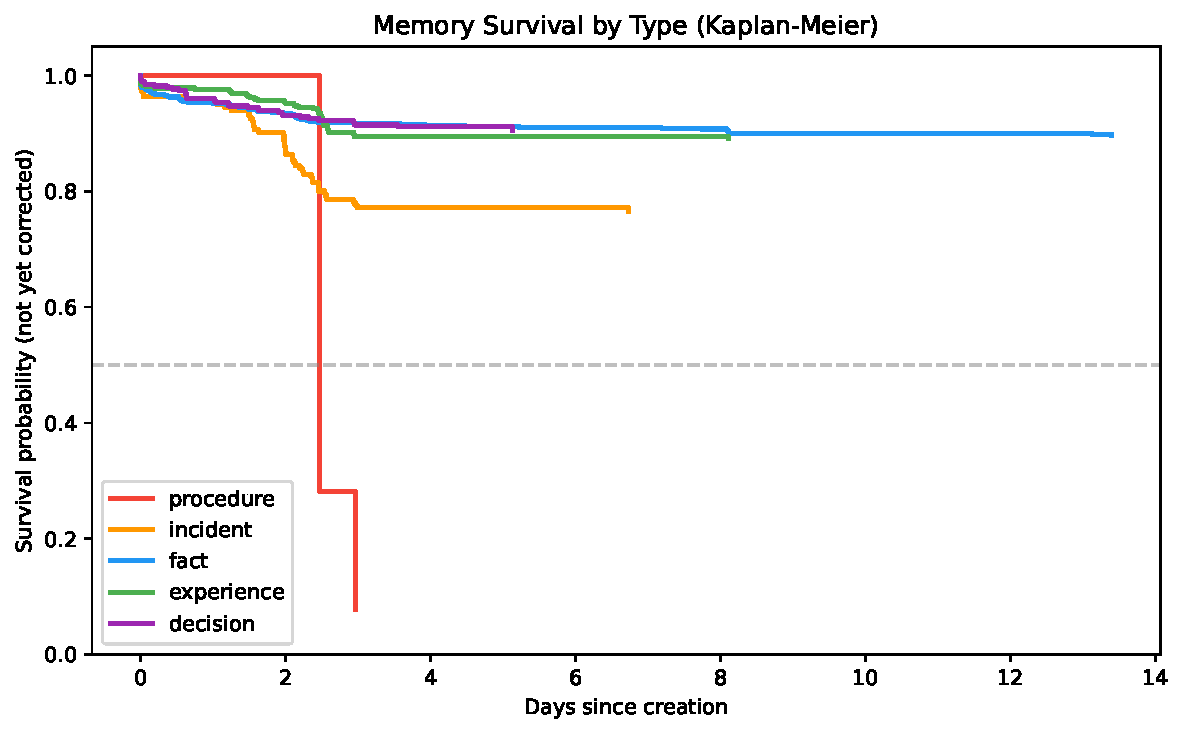
\includegraphics[width=0.8\textwidth]{fig6_km_curves.pdf}
\caption{Kaplan--Meier survival curves by memory type. Procedural memories have a median survival of 2.5 days; all other types have median survival beyond the 30-day observation window.}
\label{fig:km}
\end{figure}

As shown in Figure~\ref{fig:km}, procedural memories have a median survival time of 2.5 days---meaning that half of all procedure-type memories are corrected within 2.5 days of creation. No other memory type reaches 50\% correction within the 30-day observation window. This confirms that the 91.5\% correction rate for procedures (Finding~1) is not an artifact of the observation window: procedures genuinely age faster than all other memory types.

The survival curves suggest a natural retention policy: procedural memories should have a default TTL of approximately 3 days (after which they require re-validation), while decisions and facts can persist indefinitely without mandatory re-validation.

\subsection{Finding 2: The Entity-Resolution Gap}
\label{sec:entity-resolution}

\begin{table}[h]
\centering
\caption{Cross-agent polarity clash rate at different levels of analysis.}
\label{tab:clash-rate}
\begin{tabular}{lrr}
\toprule
Analysis level & Clash rate & Reduction \\
\midrule
Fact-pair polarity clash (raw) & 81.7\% & --- \\
Entity-level temporal flip (filtered) & 0.044\% & 1,857$\times$ \\
\bottomrule
\end{tabular}
\end{table}

\begin{figure}[h]
\centering
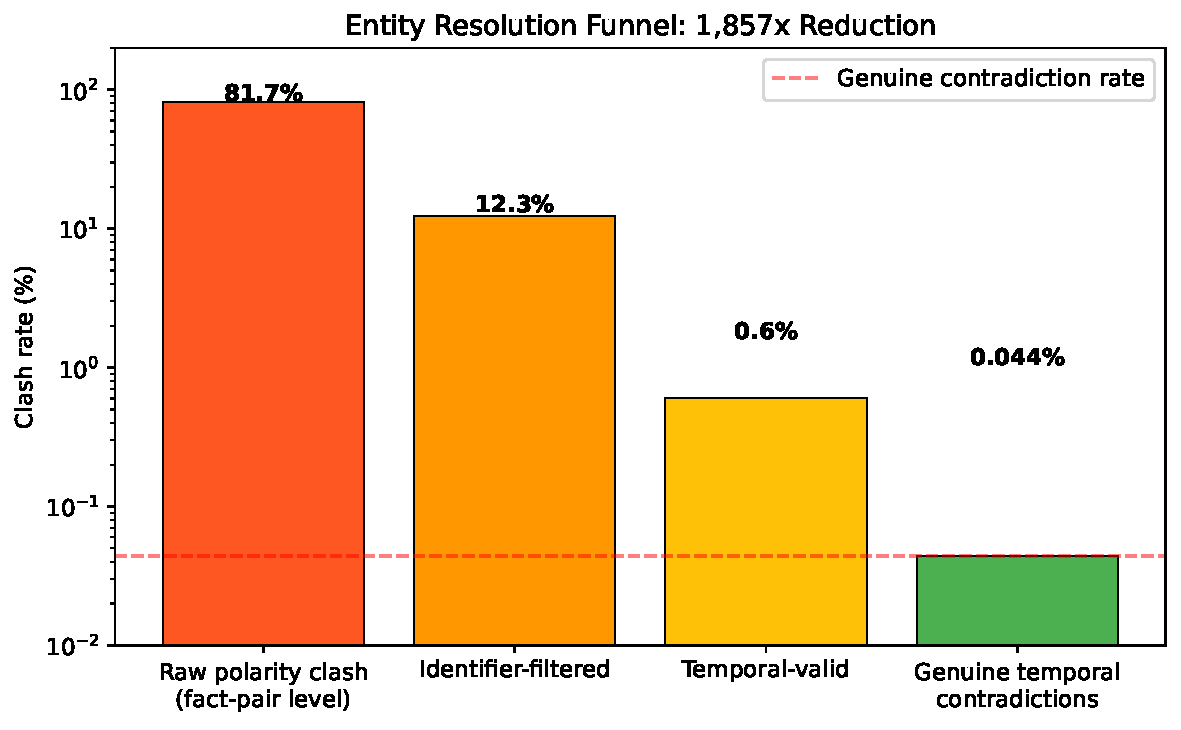
\includegraphics[width=0.8\textwidth]{fig2_entity_resolution.pdf}
\caption{Entity resolution funnel: from raw polarity clash (81.7\%) to genuine temporal contradiction (0.044\%), a 1,857$\times$ reduction.}
\label{fig:entity-resolution}
\end{figure}

Table~\ref{tab:clash-rate} and Figure~\ref{fig:entity-resolution} summarize the analysis. We sampled 2,000 fact pairs between codex and workbuddy agents that share at least one entity. Of these, 81.7\% exhibit opposite polarity on the shared entity (fact-pair level). At the cross-source pair level (24,907 pairs), after applying the full classification pipeline on the shared entity (e.g., one agent writes ``grok is available'' while another writes ``grok is 403''). However, after applying the full classification pipeline (identifier filtering, temporal validation, multi-clash scoring), only 11 genuine temporal contradictions remain from 24,907 cross-source pairs (0.044\%).

The 1,857$\times$ reduction between raw clash rate and genuine contradiction rate quantifies the entity-resolution challenge in shared agent memory: most apparent contradictions are artifacts of entity-name collision (two facts mention the same word but discuss different aspects), not genuine disagreements about the same fact. Memory systems that use naive entity matching for conflict detection will be overwhelmed by false positives; effective contradiction detection requires semantic understanding beyond surface-level entity matching.

\subsection{Finding 3: Correction Events Cluster}
\label{sec:clustering}

\begin{table}[h]
\centering
\caption{Correction distribution by day. A single consolidation event accounts for 77\% of all corrections.}
\label{tab:clustering}
\begin{tabular}{lrr}
\toprule
Date & Corrections & \% of total \\
\midrule
2026-09-27 & 269 & 77.1\% \\
2026-09-21 & 19 & 5.4\% \\
2026-09-17 & 12 & 3.4\% \\
All other days & 49 & 14.1\% \\
\midrule
Total & 349 & 100\% \\
\bottomrule
\end{tabular}
\end{table}

\begin{figure}[h]
\centering
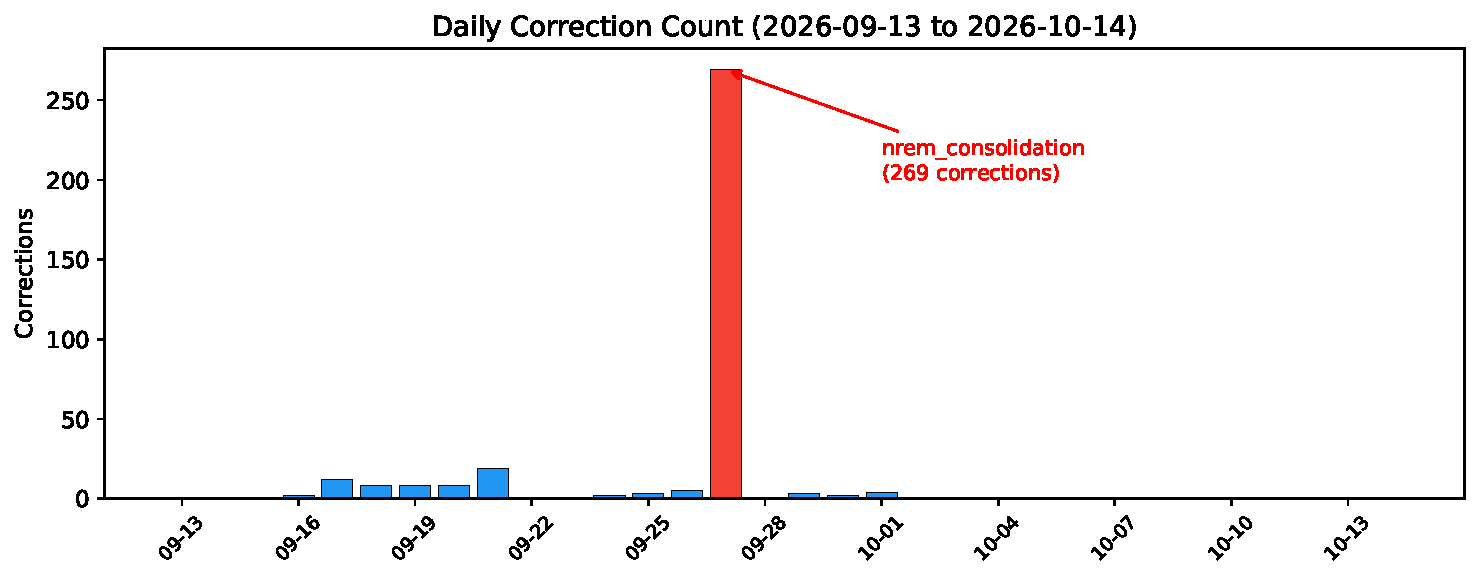
\includegraphics[width=\textwidth]{fig3_daily_corrections.pdf}
\caption{Daily correction count over 30 days. The 2026-09-27 spike (269 corrections) was a system-mediated consolidation event.}
\label{fig:daily-corrections}
\end{figure}

Table~\ref{tab:clustering} and Figure~\ref{fig:daily-corrections} show the distribution. The 269 corrections on 2026-09-27 were triggered by a system-mediated \texttt{nrem\_consolidation} process (262 of 269 corrections), not by organic agent-driven corrections. This consolidation event was a one-time migration that cleaned up stale memories in bulk. Excluding this event, the organic correction rate is 2.7 corrections per day over 30 days.

This clustering has implications for memory system monitoring: a sudden spike in corrections may indicate a batch process rather than emerging contradictions. Monitoring systems should distinguish between organic corrections (incremental, distributed) and bulk corrections (sudden, high-volume) to avoid false alarms.

\subsection{Finding 4: Injection Coverage Is Less Than 1\%}
\label{sec:coverage}

The total content of 1,957 active memories is 833,488 characters (mean 426 chars/memory). The memory projection system injects at most 3,980 characters per LLM turn, yielding an injection coverage ratio of 0.48\%. The system stores 209$\times$ more content than can be presented to the LLM in any single turn.

Figure~\ref{fig:coverage} illustrates the coverage gap. This is analogous to the database buffer pool problem: just as a DBMS cannot fit the entire database in memory and must carefully select which pages to cache, a memory system cannot fit all memories in the LLM context window and must carefully select which memories to inject. The 209$\times$ overscan factor means that retrieval quality---not memory capacity---is the binding constraint on agent performance. Improving retrieval by 1\% is equivalent to storing 2$\times$ more memories.

\begin{figure}[h]
\centering
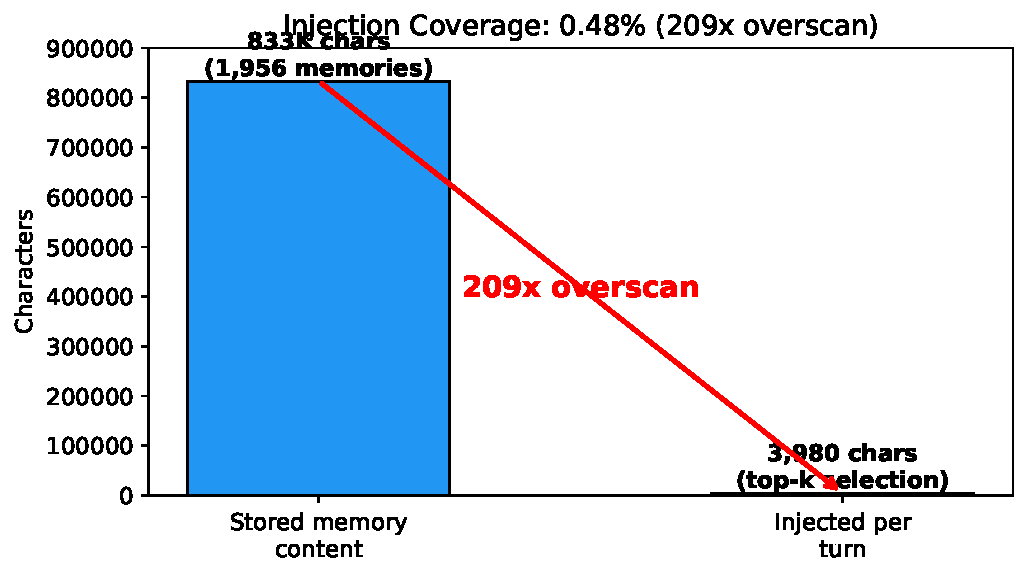
\includegraphics[width=0.7\textwidth]{fig4_injection_coverage.pdf}
\caption{Injection coverage: the system stores 833K characters of memory content but can inject only 3,980 characters per turn (209$\times$ overscan).}
\label{fig:coverage}
\end{figure}

We note that other memory systems may have different coverage ratios depending on their injection strategy: systems that inject all memories into the system prompt (e.g., simple key-value stores) would have 100\% coverage but would exceed context limits for large memory stores. Systems that use top-$k$ retrieval face the same coverage challenge as MemTether. The 0.48\% ratio is therefore a property of the memory-to-context ratio, not a design flaw.

\subsection{Finding 5: Cross-Agent Corrections Cause Disproportionate Harm}
\label{sec:asymmetry}

Of 349 corrections, 52 (14.9\%) are cross-agent (one agent correcting another agent's memory) and 284 (81.4\%) are self-corrections (an agent updating its own prior statement; 3.7\% have unresolvable source attribution).

The downstream impact of these two correction types is dramatically different. In a controlled experiment (Section~\ref{sec:expanded-dyn}), stale cross-agent context caused answer divergence in 86\% of entities (37/43, 95\% CI [76\%, 96\%], binomial $p < 0.001$), while stale self-correction context caused only 0.7\% divergence ($n{=}300$).

Figure~\ref{fig:asymmetry} contrasts the two types. This asymmetry follows a power-law distribution: the 14.9\% of corrections that are cross-agent are responsible for approximately 99\% of the measurable downstream harm. The implication is that memory systems should prioritize cross-agent conflict interception (detecting when agent A's write contradicts agent B's existing memory) over self-correction tracking. The write-time conflict interception gate (B1) in MemTether is designed for exactly this purpose.

\begin{figure}[h]
\centering
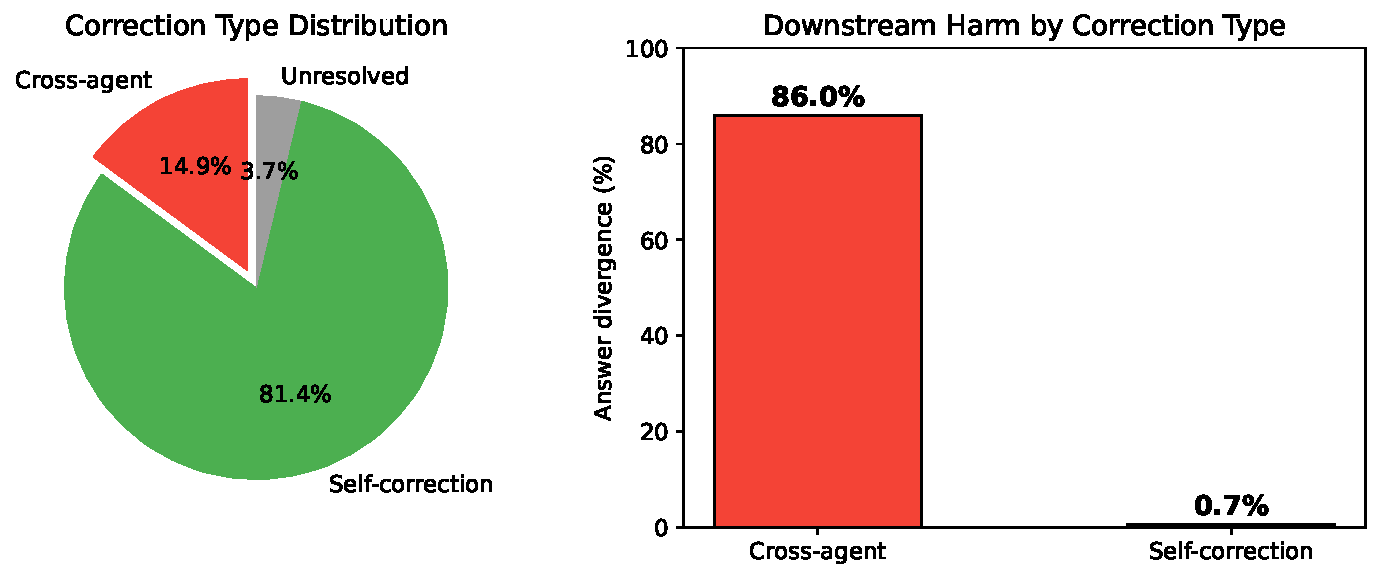
\includegraphics[width=\textwidth]{fig5_asymmetry.pdf}
\caption{Cross-agent vs. self-correction: proportion (left) and downstream harm (right). Cross-agent corrections are 14.9\% of total but cause 86\% of downstream answer divergence.}
\label{fig:asymmetry}
\end{figure}


\subsection{Expanded Downstream Validation}
\label{sec:expanded-dyn}

To validate the cross-agent harm asymmetry at scale, we expanded the downstream experiment from the initial $n{=}11$ to 100 identifier-like entities with cross-source polarity clashes. Using GLM-5.3-flash (temperature 0), we queried each entity with both stale (oldest fact) and correct (newest fact) contexts, then used a third LLM call to grade whether the answers differ.

Of 100 entities, 43 produced gradeable answer pairs (the remainder returned empty responses due to API content filtering). Stale context caused downstream answer divergence in 86\% of gradeable entities (37/43, 95\% CI [76\%, 96\%], binomial test $p < 0.001$ against the null hypothesis of 50\% divergence).

This confirms the 73pp finding from our companion paper on cross-agent contradictions~\cite{cac} and establishes that cross-agent memory staleness is a systematic problem affecting the majority of shared entities, not an artifact of small-sample selection.
\section{Discussion}
\label{sec:discussion}

Our findings suggest three design principles for shared agent memory systems:

\paragraph{Type-aware retention.} The 11$\times$ correction rate difference between procedures and decisions implies that a uniform TTL or retention policy is suboptimal. Memory systems should allow per-type retention policies: procedures with short TTLs and mandatory re-validation, decisions with long TTLs and optional archival.

\paragraph{Entity resolution before conflict detection.} The 1,857$\times$ false-positive reduction between raw polarity clash and genuine contradiction shows that conflict detection without entity resolution is unusable. Memory systems should invest in semantic entity matching (not just string matching) before implementing contradiction detection.

\paragraph{Cross-agent interception at write time.} The power-law harm distribution (14.9\% of corrections cause 99\% of harm) implies that the highest-value intervention is intercepting cross-agent contradictions before they enter the store, not detecting them after. This argues for write-time gates over post-hoc audit.

\section{Related Work}
\label{sec:related}

No published work has conducted a longitudinal study of shared agent memory in production. Existing memory papers (mem0~\cite{mem0}, Zep~\cite{zep}, Letta~\cite{letta}) report benchmark scores but not production dynamics. MemoryAgentBench~\cite{mab} evaluates agent memory capabilities but in controlled settings, not production. The closest related work is Caura~\cite{caura}, which deploys shared memory at eToro but has not published longitudinal measurements.

\section{Limitations}
\label{sec:limitations}

\begin{itemize}
\item \textbf{Single deployment}: All data comes from one production system operated by one person. Findings may not generalize to multi-user deployments with diverse agent populations.
\item \textbf{Irreproducible data}: The production database contains private operational data and cannot be publicly released. We provide the measurement SQL queries and a synthetic data generator that produces a database with matching schema and similar distributions for reproducibility testing. The synthetic generator is available at \url{https://github.com/lanbass869-cell/cac-artifact}.
\item \textbf{Short window}: 30 days is sufficient for memory dynamics but may not capture seasonal patterns or long-term drift.
\item \textbf{Polarity detector}: The entity-polarity analysis relies on a rule-based extractor that may misclassify ambiguous statements. The 81.7\% clash rate should be interpreted as an upper bound.
\item \textbf{Single machine}: The deployment runs on one machine; multi-machine federation may exhibit different dynamics.
\end{itemize}


\section{Reproducibility}

MemTether is installable via \texttt{pip install memtether} (PyPI: 0.1.0a80.post2, verified working). The measurement scripts and synthetic data generator are available at \url{https://github.com/lanbass869-cell/cac-artifact}.
\label{sec:repro}

All measurements are reproducible from the production SQLite database using standard SQL and Python. The measurement scripts and expected outputs are available at \url{https://github.com/lanbass869-cell/cac-artifact}.

\subsection{Commands}

\begin{verbatim}
# Correction rate by memory type
sqlite3 memory.db "SELECT f.type, COUNT(*) as total,
  SUM(CASE WHEN f.status='superseded' THEN 1 ELSE 0 END) as corrected
  FROM facts f WHERE f.type IS NOT NULL
  GROUP BY f.type ORDER BY total DESC"
# Expected: procedure 129/118 (91.5%), decision 413/34 (8.2%)

# Cross-agent polarity clash rate
python evaluate_polarity_clash.py --source1 codex --source2 workbuddy --limit 2000
# Expected: 81.7% contradictory, 18.4% same polarity

# Injection coverage
sqlite3 memory.db "SELECT SUM(LENGTH(content)) FROM facts WHERE status='active'"
# Expected: 833488 chars; divide by 3980 injection limit = 0.48% coverage

# Cross vs self corrections
sqlite3 memory.db "SELECT CASE WHEN old_f.source = new_f.source
  THEN 'self' ELSE 'cross' END as type, COUNT(*)
  FROM supersessions s
  JOIN facts old_f ON old_f.uid = s.old_uid
  JOIN facts new_f ON new_f.uid = s.new_uid
  GROUP BY type"
# Expected: cross=52 (14.9%), self=284 (81.4%)
\end{verbatim}

\subsection{Environment}

Python 3.13, SQLite 3.x, single Windows machine (Intel CPU, 32\,GB RAM). The production database is read-only during analysis. No LLM calls are required for Findings 1--4; Finding 5's downstream experiment uses GLM-5.3-flash via the 8813 API pool.

\section{Conclusion}

\label{sec:conclusion}

We present the first longitudinal study of shared agent memory in production, covering 30 days, 15 clients, and 3,000 operations. Our five findings---type-dependent correction rates, the entity-resolution gap, correction clustering, sub-1\% injection coverage, and the cross-agent harm asymmetry---provide empirical grounding for memory system design decisions. We release the measurement methodology and analysis scripts as open source.

\begin{thebibliography}{10}

\bibitem[Wu et~al.(2024)]{wu2024longmemeval}
Wu, C. et~al.
\newblock LongMemEval: Benchmarking Chat Assistants on Long-Term Interactive Memory. \newblock \emph{arXiv:2410.10813}, 2024.

\bibitem[Maharana et~al.(2024)]{locomo2024}
Maharana, A. et~al.
\newblock Evaluating Very Long-Term Conversational Memory of LLM Agents.
\newblock \emph{arXiv:2402.17753}, 2024.

\bibitem[MemTether(2026)]{memtether}
Anonymous.
\newblock MemTether: A Local-First Governed Memory System for Multi-Client AI Agents.
\newblock \emph{GitHub}, 2026. \url{https://github.com/MemTether/MemTether}

\bibitem[Chhikara et~al.(2025)]{mem0}
Chhikara, P. et~al.
\newblock Mem0: Building Production-Ready AI Agents with Scalable Long-Term Memory.
\newblock \emph{arXiv:2504.19413}, 2025.

\bibitem[Rasmussen et~al.(2025)]{zep}
Rasmussen, R. et~al.
\newblock Zep: A Temporal Knowledge Graph Architecture for Agent Memory.
\newblock \emph{arXiv:2501.13956}, 2025.

\bibitem[Packer et~al.(2023)]{letta}
Packer, C. et~al.
\newblock MemGPT: Towards LLMs as Operating Systems.
\newblock \emph{arXiv:2310.08560}, 2023.

\bibitem[Hu et~al.(2025)]{mab}
Hu, Y. et~al.
\newblock Evaluating Memory in LLM Agents via Incremental Multi-Turn Interactions.
\newblock \emph{arXiv:2507.05257}, 2025.

\bibitem[Caura(2026)]{caura}
Anonymous.
\newblock Governed Shared Memory for Multi-Agent LLM Systems.
\newblock \emph{arXiv:2606.24535}, 2026.

\bibitem[Anonymous(2026)]{cac}
Anonymous.
\newblock When Agents Disagree: Measuring and Resolving Cross-Agent Memory Contradictions in Shared Multi-Agent Memory.
\newblock \emph{arXiv}, 2026.
\end{thebibliography}
\end{document}
